\documentclass[letterpaper,openany,twoside,twocolumn]{book}

\newcommand{\PATH}{../../../../}

\usepackage{\PATH templates/utilities/image-db}
\usepackage{\PATH templates/utilities/m4rz-fonts}
\usepackage{\PATH templates/utilities/m4rz-colors}
\usepackage{\PATH templates/utilities/miscellaneous}
\usepackage{\PATH templates/utilities/shadowfy}

\usepackage[justified]{\PATH templates/template_dnd/dnd}

\usepackage{\PATH templates/template_book/book_commands}


\usepackage{\PATH templates/template_adventure/adventure_commands}
\usepackage{\PATH templates/template_dungeon/dungeon_commands}
\usepackage{\PATH templates/template_monster/monster_commands}
%\usepackage[edition=5e24]{\PATH templates/template_character-sheet/character-sheet-stylesheet} FAULTY INPUT?
\usepackage{\PATH templates/template_magic-item/magic-items_commands}
\usepackage{\PATH templates/template_resource/resource_commands}


\graphicspath{{.././images}}

\newrefformat{or}{\hyperref[#1]{\LinkFont{Optional Rule \ifnumcomp{\getrefnumber{#1}}<10{0}{}\ref{#1}}}}

\begin{document}
	\DndSetThemeColor[PhbTan]
	
	\eject \pdfpagewidth=12in \pdfpageheight=12in \thispagestyle{empty}
	\begin{tikzpicture}[remember picture, overlay]%
		\node[opacity=1, inner sep=0pt, xshift=4.5cm, yshift=1.3cm] at (current page.center){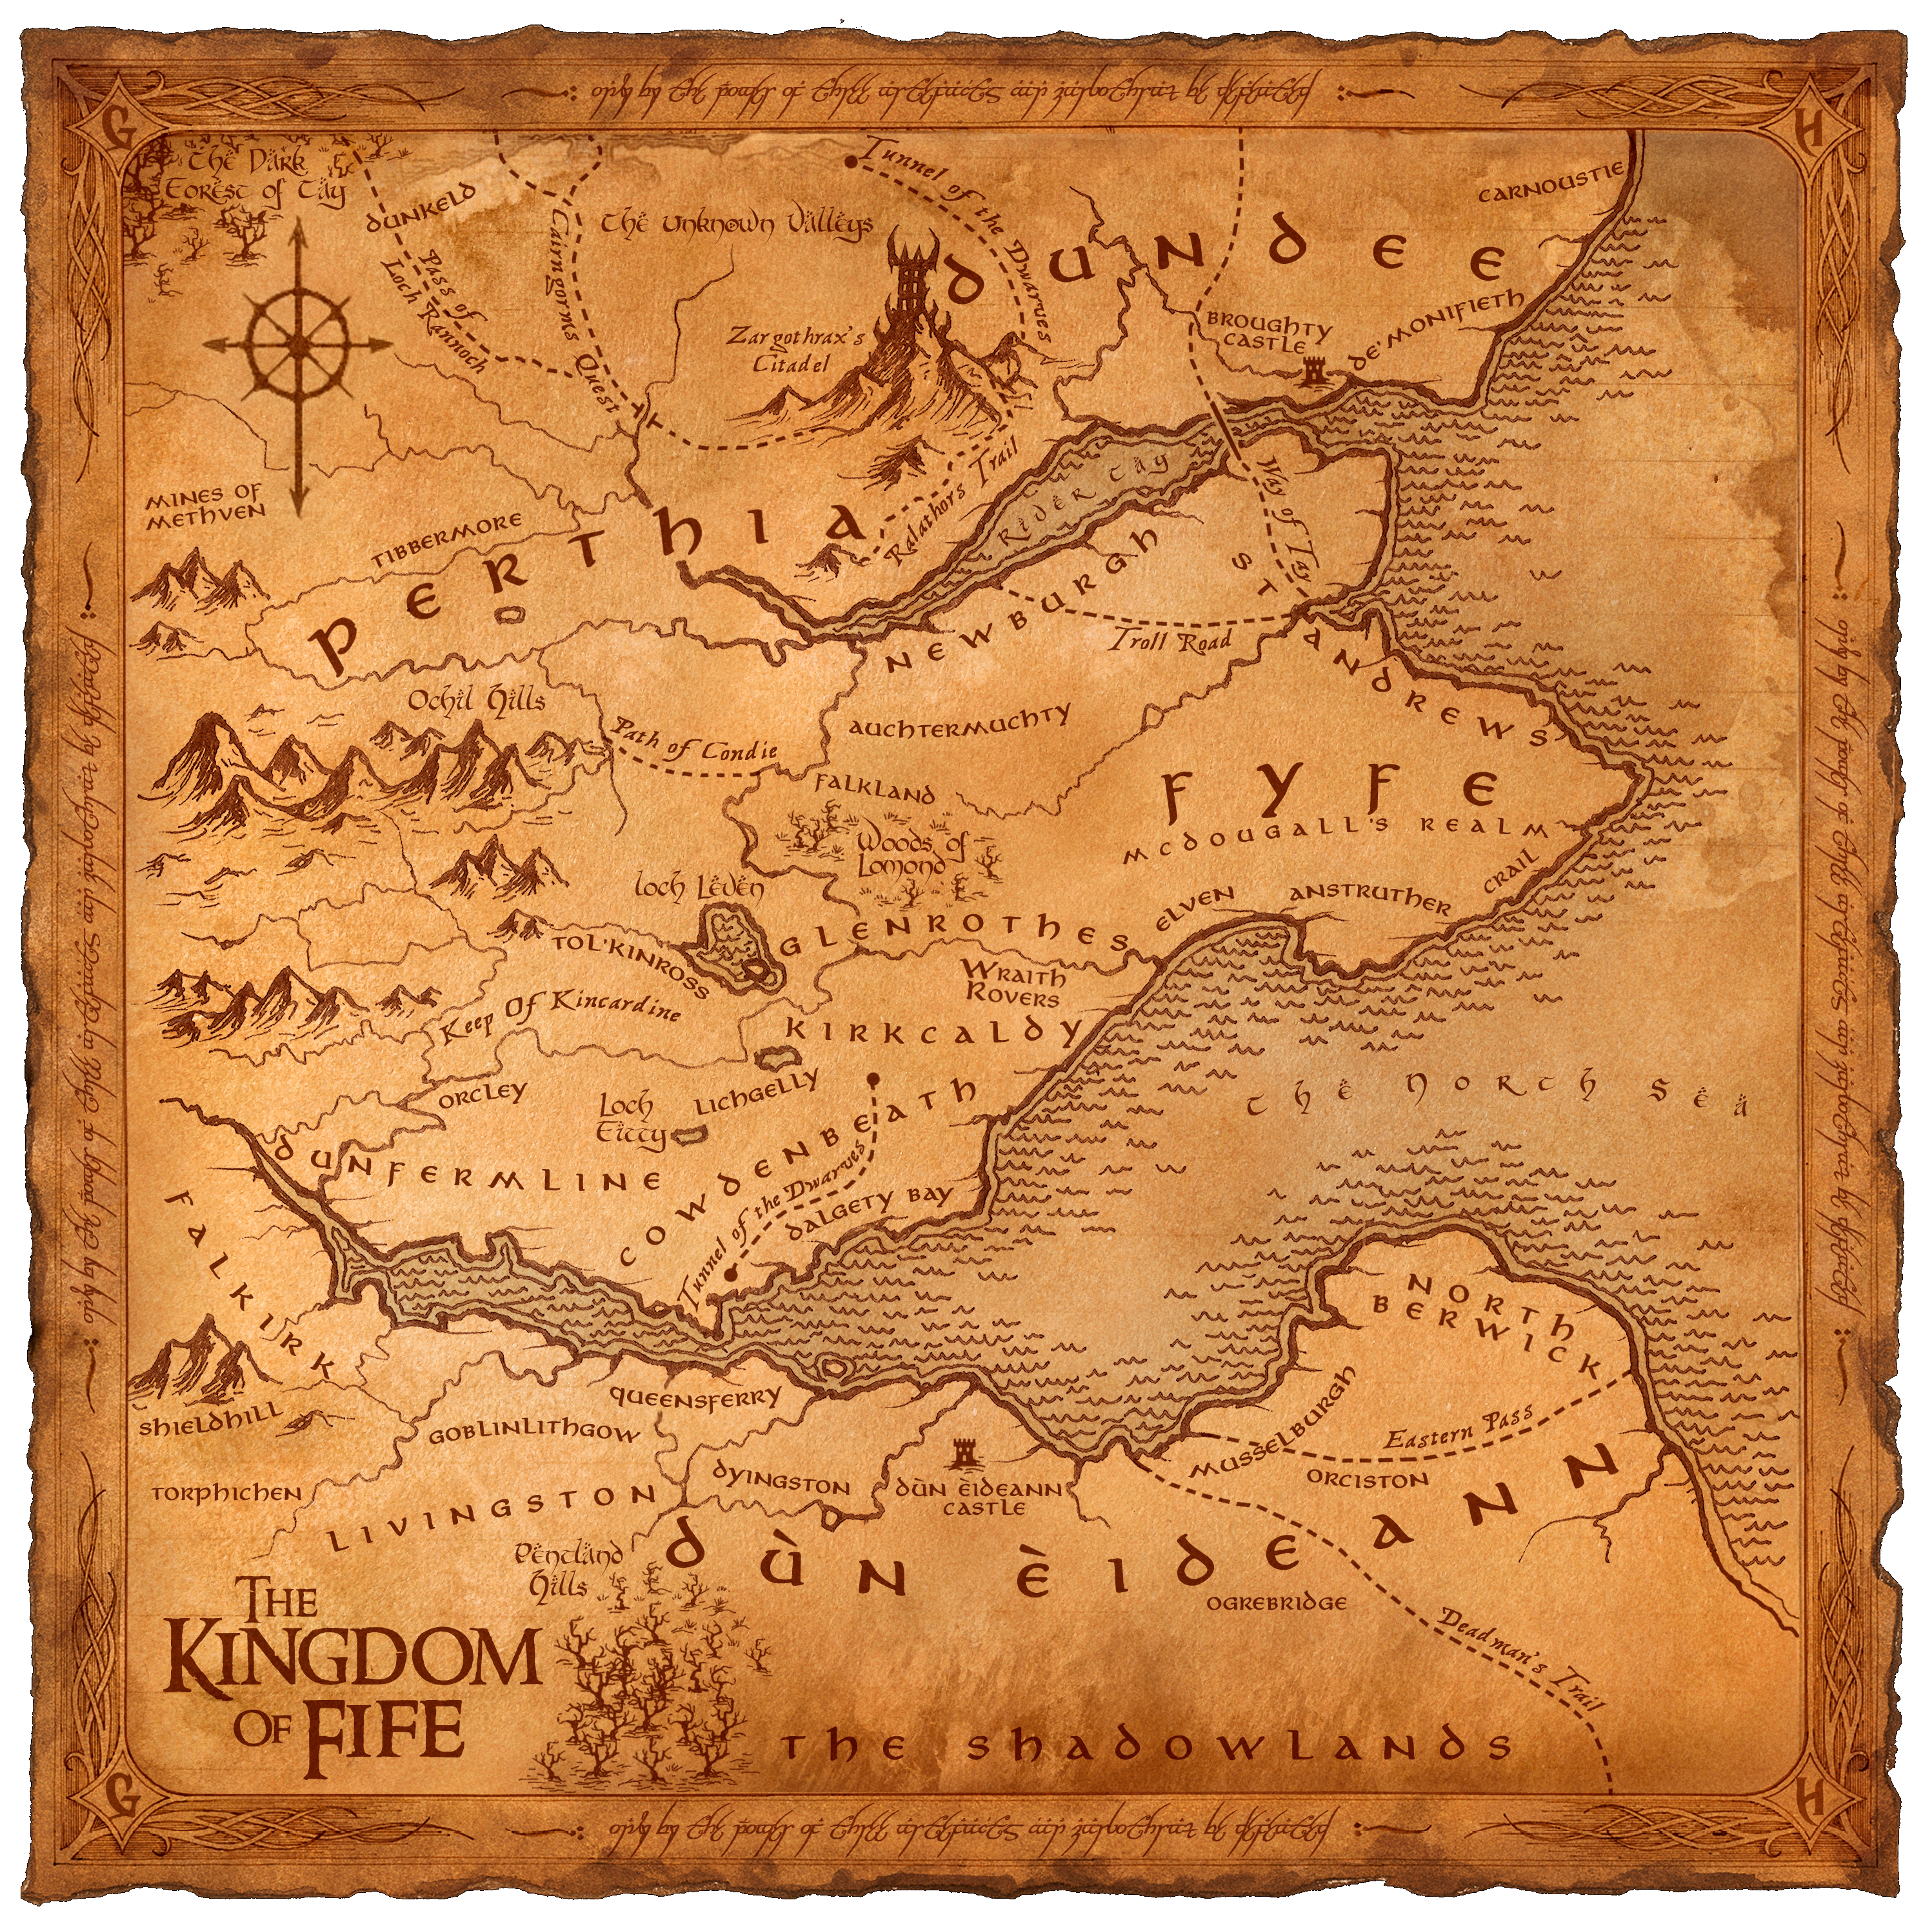
\includegraphics[width=12.65in, keepaspectratio]{Kingdom_of_Fife_Map.png}};%
		
		% 0 - 110
		\begin{scope}[scale=0.25, xshift=-4cm, yshift=-110cm]			
			% Travel Routes
			\draw[line width=3pt, blue] (70,95) -- (78,78) -- (85,75) -- (95,60);
			\draw[line width=3pt, red] (95,60) -- (88,63);
			
			% Known PoIs
			\pgfmathsetmacro{\IndicatorSize}{15*\scaleFactor}%
			\indicatorAlphField[10]{(70,95)}{\IndicatorSize}; % Dundee
			\indicatorAlphField[10]{(95,60)}{\IndicatorSize}; % Citadel of Crail
			\indicatorAlphField[10]{(5,80)}{\IndicatorSize}; % Mines of Methven
			\indicatorAlphField[10]{(18,106)}{\IndicatorSize}; % Dunkeld
			\indicatorAlphField[10]{(50,47)}{\IndicatorSize}\indicatorAddition[!]{(50,47)}{\IndicatorSize}; % Auchtertool
			
			% Home Cities
			\pgfmathsetmacro{\IndicatorSize}{10*\scaleFactor}%
			\indicatorLowerCaseAlphField[10]{(75,110)}{\IndicatorSize}\indicatorAddition[$\uparrow$]{(75,110)}{\IndicatorSize}; % Aberdeen
			\indicatorLowerCaseAlphField[10]{(33,7)}{\IndicatorSize}
			
			% Possible PoIs / Rumors
			\pgfmathsetmacro{\IndicatorSize}{13*\scaleFactor}%
			\indicatorNumberField[10]{(82,78)}{\IndicatorSize}\indicatorAddition[?]{(82,78)}{\IndicatorSize};
			\indicatorNumberField[10]{(88,63)}{\IndicatorSize};
			\indicatorNumberField[10]{(47,63)}{\IndicatorSize}\indicatorAddition[?]{(47,63)}{\IndicatorSize};
			\indicatorNumberField[10]{(55,70)}{\IndicatorSize}\indicatorAddition[?]{(55,70)}{\IndicatorSize};
			\indicatorNumberField[10]{(2,40)}{\IndicatorSize}\indicatorAddition[$\swarrow$]{(2,40)}{\IndicatorSize};
		\end{scope}
	\end{tikzpicture}%
	\clearpage
	\eject \pdfpagewidth=12in \pdfpageheight=13.75in \thispagestyle{empty}
	\begin{tikzpicture}[remember picture, overlay]%
		\node[opacity=1, inner sep=0pt, xshift=4.5cm, yshift=3.5cm] at (current page.center){\includegraphics[width=12in, keepaspectratio]{Map_of_Caledonia.png}};%
		
		% 0 - 110
		\begin{scope}[scale=0.25, xshift=-4cm, yshift=-110cm]
			
			% Known PoIs
			\pgfmathsetmacro{\IndicatorSize}{12*\scaleFactor}%
			\resetIndicatorAlphCounter
			\indicatorAlphField[10]{(79,31)}{\IndicatorSize}; % Dundee
			\indicatorAlphField[10]{(84,24)}{\IndicatorSize}; % Citadel of Crail
			\indicatorAlphField[10]{(66,28)}{\IndicatorSize}; % Mines of Methven
			\indicatorAlphField[10]{(72,33)}{\IndicatorSize}; % Dunkeld
			\indicatorAlphField[10]{(74,22)}{\IndicatorSize}; % Auchtertool
			
			% Home Cities
			\pgfmathsetmacro{\IndicatorSize}{10*\scaleFactor}%
			\resetIndicatorLowerCaseAlphCounter
			\indicatorLowerCaseAlphField[10]{(91,51)}{\IndicatorSize}; % Aberdeen
			\indicatorLowerCaseAlphField[10]{(73,11)}{\IndicatorSize};
			
			% Possible PoIs / Rumors
			\pgfmathsetmacro{\IndicatorSize}{10*\scaleFactor}%
			\resetIndicatorCounter
			\stepcounter{indicatorNumber}%\indicatorNumberField[10]{(82,78)}{\IndicatorSize};
			\stepcounter{indicatorNumber}%\indicatorNumberField[10]{(88,63)}{\IndicatorSize};
			\stepcounter{indicatorNumber}%\indicatorNumberField[10]{(47,63)}{\IndicatorSize};
			\stepcounter{indicatorNumber}%\indicatorNumberField[10]{(55,70)}{\IndicatorSize};
			\indicatorNumberField[10]{(58,13)}{\IndicatorSize};
		\end{scope}
	\end{tikzpicture}%
	\clearpage
	\eject \pdfpagewidth=\paperwidth \pdfpageheight=\paperheight \thispagestyle{fancy}
	\chapter*{Points-of-Interest Map}
	\subsection*{Larger Settlements / Cities}
	\inTextCircled[10]{A}{10} {\entryfont The (once) great city of Dundee}\\
	\inTextCircled[10]{B}{10} {\entryfont Citadel of Crail}\\
	\inTextCircled[10]{C}{10} {\entryfont Mines of Methven}\\
	\inTextCircled[10]{D}{10} {\entryfont Dunkeld}\\
	\inTextCircled[10]{E}{10} {\entryfont Auchtertool}
	\subsubsection*{Home Cities}
	\inTextCircled[10]{a}{10} {\entryfont Aberdeen (3 days travel from Dundee)}\\
	\inTextCircled[10]{b}{10} {\entryfont Sylvani Elves Village}\\
	\subsection*{Landmarks and Locations}
	\inTextCircled[10]{1}{10} {\entryfont River Maiden Wreckage}\\
	\inTextCircled[10]{2}{10} {\entryfont Eagle's Peak}\\
	\inTextCircled[10]{3}{10} {\entryfont Elven Village}\\
	\inTextCircled[10]{4}{10} {\entryfont Auchtermuchty}\\
	\inTextCircled[10]{5}{10} {\entryfont Swamps of Paisley (3 days travel from Auchtertool)}\\
\end{document}